\chapter{Physical testing of prepreg material}
\label{physical}

\section{Ply thickness}
\label{sec:plythick}

Ply thickness will be measured using 10 random points in the laminate after curing and before specimen cutting. It'll allow us to determine if the laminate is consistent in its full extent, as well as determine if there's defects in the laminate. Normalized cured ply thickness and/or fiber volume fraction will be used for most lamina level tension and compression strength and modulus properties normalization. Lamina level properties that wont be normalized include in-plane shear strength, modulus and Poisson's ratio, since data scatter should reduce or remain the same. If data scatter increases significantly after normalizing, the reason must be investigated. Wherever properties are normalized, both measured and normalized data will be considered.

The 10 thickness measurements in each group of panels with the same number of plies and utilizing the formulation presented below. The same procedure ought to be done to test specimens as well, however performing 3 measurements instead of 10. The nominal ply thickness is calculates using the following expression:

\begin{equation}
\label{eq:nominal}
\gls{npt} = \left(  \frac{\frac{t_{1}}{\gls{npp}}+\frac{t_{2}}{\gls{npp}}+\frac{t_{3}}{\gls{npp}}+...+\frac{\gls{ti}}{\gls{npp}}}{\gls{nm}} \right)
\end{equation}

In accordance with equation \ref{eq:normalized}, the average nominal thickness from the panels is used to obtain the nominal thickness:

\begin{equation}
\label{eq:normalized}
\gls{tn} = \frac{\sum \gls{tpi}}{\gls{np}}
\end{equation}


\subsection{Procedure}
\label{ply:procedure}

To accurately measure the laminate, a micrometer is advised. However, in some cases, to accurately measure a more complex laminate, a specific micrometer was used, as shown in figure \ref{fig:micrometers}

\begin{figure}[htbp]
\centering
\quad
 \subbottom[Regular micrometer measuring]{%
    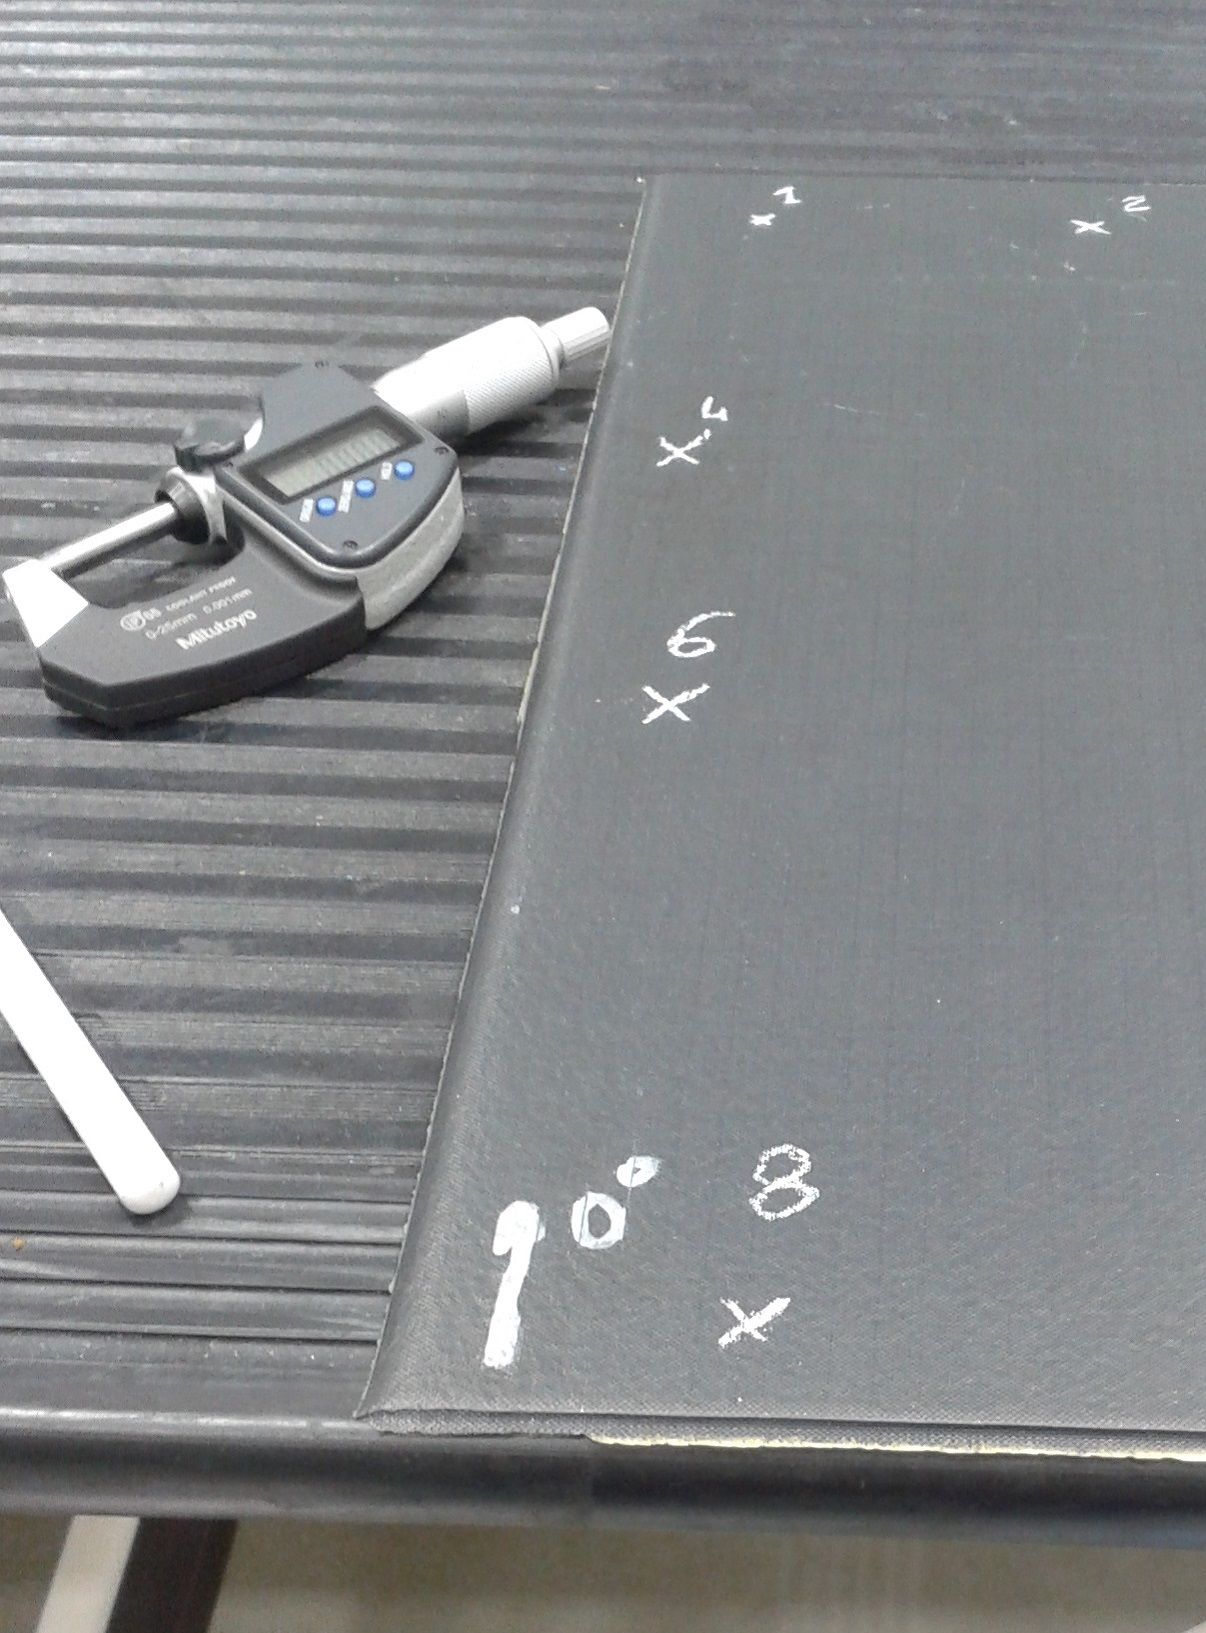
\includegraphics[width=0.35\linewidth]{micrometer}}%
    \quad
 \subbottom[Larger micrometer measuring]{%
    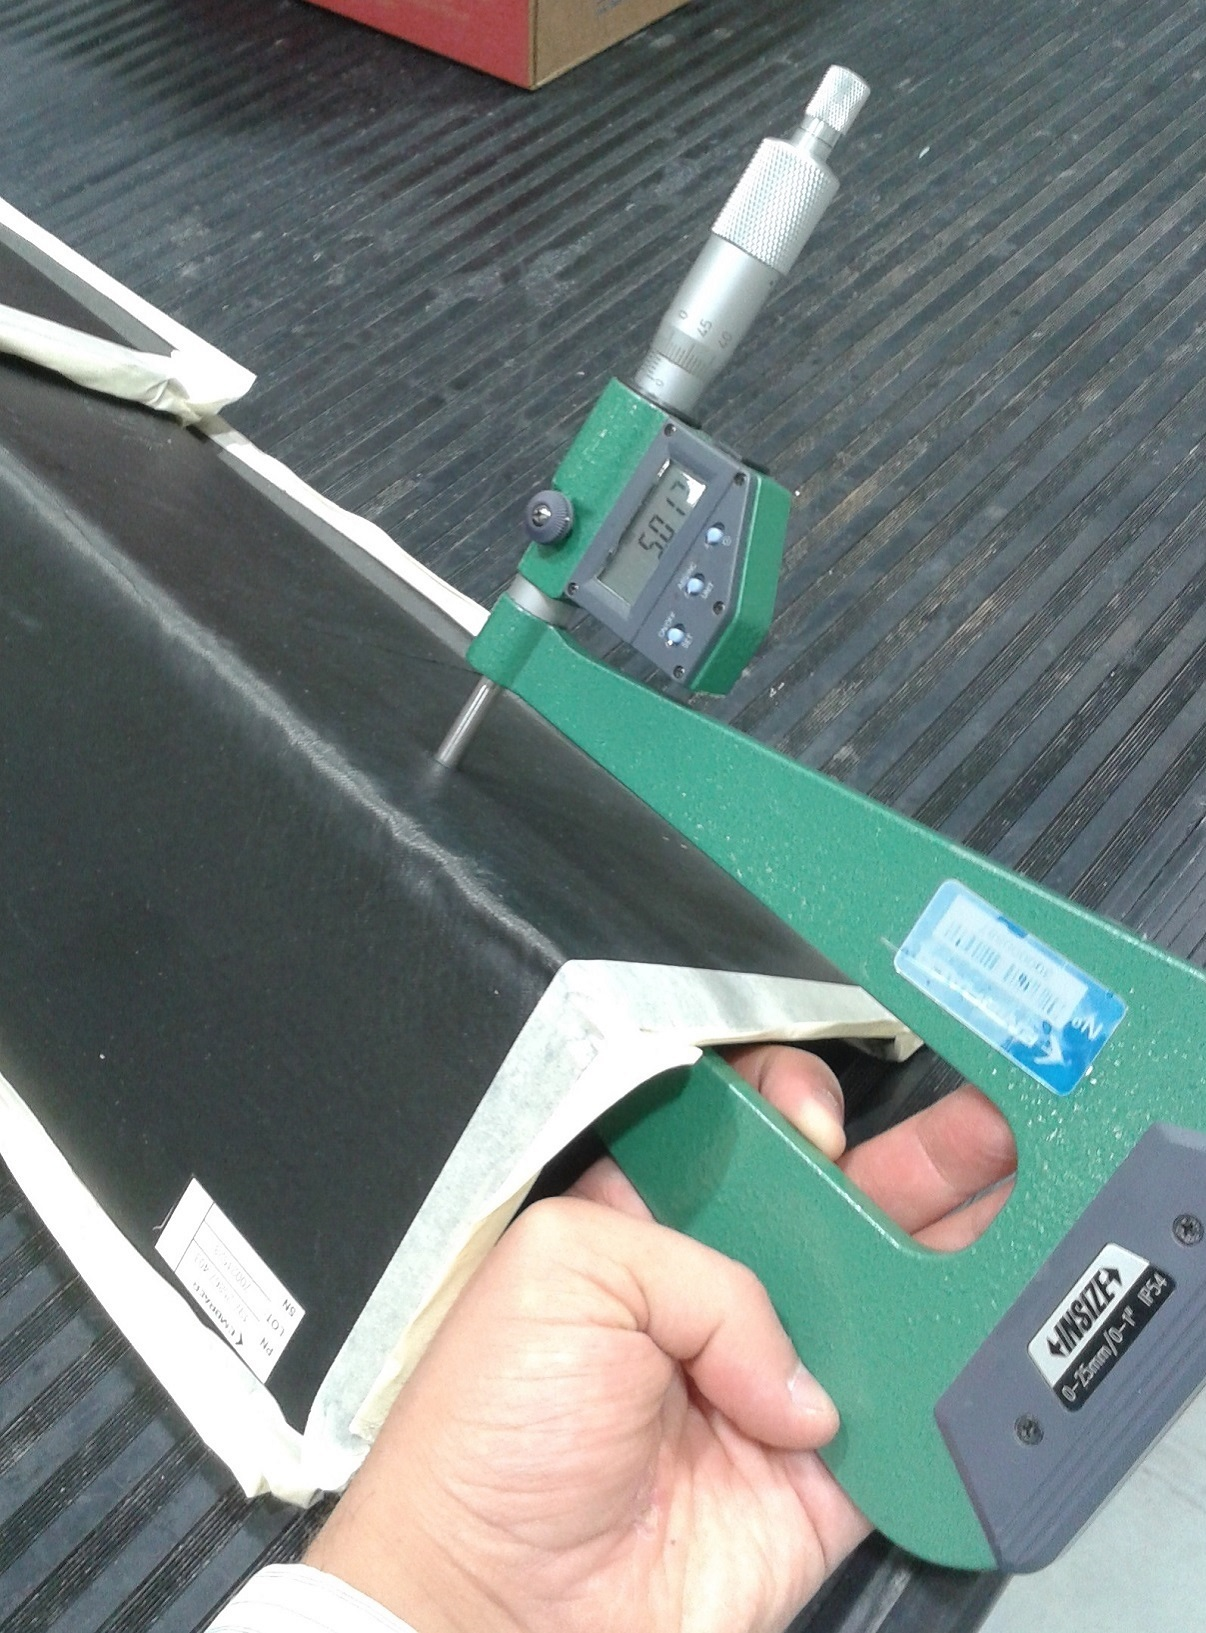
\includegraphics[width=0.35\linewidth]{largermicrometer}}
\caption{Micrometer measuring for calculating Normalized Ply Thickness.}
\label{fig:micrometers}
\end{figure}

\subsection{Results and discussion}
\label{ply:results}

\section{Fourier Transform Infrared}
\label{sec:ftir}

\gls{ftir} it will be used to evaluate the material in a whole, regarding the eventual inclusions and impurities present in the material. This will help us define if there's more in the prepreg than necessary, specially after hot drape. Although there are measure to prevent it, there may be some exchange of material between the prepreg and the hot drape screen.

\subsection{Procedure}
\label{ftir:procedure}

The samples are prepared according to ASTM E168 by withdrawing the resin of the prepreg, with reagent grade methylene chloride at room temperature and then the fibers are manipulated in order to ensure full resin withdraw. The resin/reagent mix is then placed on a salt block and the solvent is evaporated. The resulted resin is then tested in a certified FTIR tester.

\subsection{Results and discussion}
\label{ftir:results}

\section{Differential Scanning Calorimetry}
\label{sec:dsc}

\texorpdfstring{\gls{dsc}}{DSC} is a thermoanalytical test to which measures the heat necessary for molecular transitions in the material to happen. In this particular thesis, DSC is going to be used to study and measure the glass transition temperature, or $T_g$, of the prepreg resin, in order to assess the purity of it as well as to guarantee its required physical properties.

\subsection{Procedure}
\label{dsc:procedure}

\subsection{Results and discussion}
\label{dsc:results}

\section{Dynamic Mechanical Analysis}
\label{sec:dma}

\cite{Menard}

\subsection{Procedure}
\label{dma:procedure}

\subsection{Results and discussion}
\label{dma:results}

